\documentclass[tikz,border=0pt]{standalone}
%% Shared style for the figures: TUHH colour palette, Latin Modern fonts.
%% Highlights are bold at caption size (10 pt); longer text is regular and
%% 2 pt smaller (8 pt). Figures are drawn at the text width of the
%% manuscript (390 pt) and must be included unscaled.
\usepackage[T1]{fontenc}
\usepackage{lmodern}
\usepackage{graphicx}
\usepackage{tikz}
\usetikzlibrary{arrows.meta,positioning,calc,fit,backgrounds}

\definecolor{tuhhturquoise}{HTML}{00C1D4}
\definecolor{tuhhyellow}{HTML}{FFDE36}
\definecolor{tuhhred}{HTML}{FF4F4F}
\definecolor{tuhhmint}{HTML}{5AFFC5}
\definecolor{tuhhcoolgray}{HTML}{D0D0CE}
\definecolor{tuhhpurple}{HTML}{7200FE}
\definecolor{tuhhwarmgray}{HTML}{A8968C}
\colorlet{ink}{black!85}

\newcommand{\hl}[1]{{\fontsize{10}{12}\selectfont\bfseries #1}}
\newcommand{\tx}[1]{{\fontsize{8}{9.6}\selectfont #1}}
\newcommand{\txi}[1]{{\fontsize{8}{9.6}\selectfont\itshape #1}}

%% \logo{file stem}{height}{fallback wordmark}: uses logos/<stem>.pdf or
%% .png when present, and a typeset wordmark otherwise.
\newcommand{\logo}[3]{%
  \IfFileExists{logos/#1.pdf}{\includegraphics[height=#2]{logos/#1.pdf}}{%
  \IfFileExists{logos/#1.png}{\includegraphics[height=#2]{logos/#1.png}}{%
  {\fontsize{10}{12}\selectfont\bfseries\sffamily #3}}}}

\tikzset{
  x=1pt, y=1pt, text=ink,
  card/.style={draw=tuhhcoolgray, line width=0.8pt, rounded corners=3pt,
               fill=white},
  band/.style={rounded corners=3pt, draw=none},
  flow/.style={-{Stealth[length=5pt,width=4.5pt]}, line width=1pt,
               draw=ink},
  gap/.style={draw=tuhhred, line width=1pt, dash pattern=on 3pt off 2pt},
  lbl/.style={inner sep=0pt, outer sep=0pt, align=left, anchor=north west},
  tag/.style={fill=tuhhyellow, rounded corners=2pt, inner xsep=3pt,
              inner ysep=1.5pt, anchor=west},
}

\begin{document}
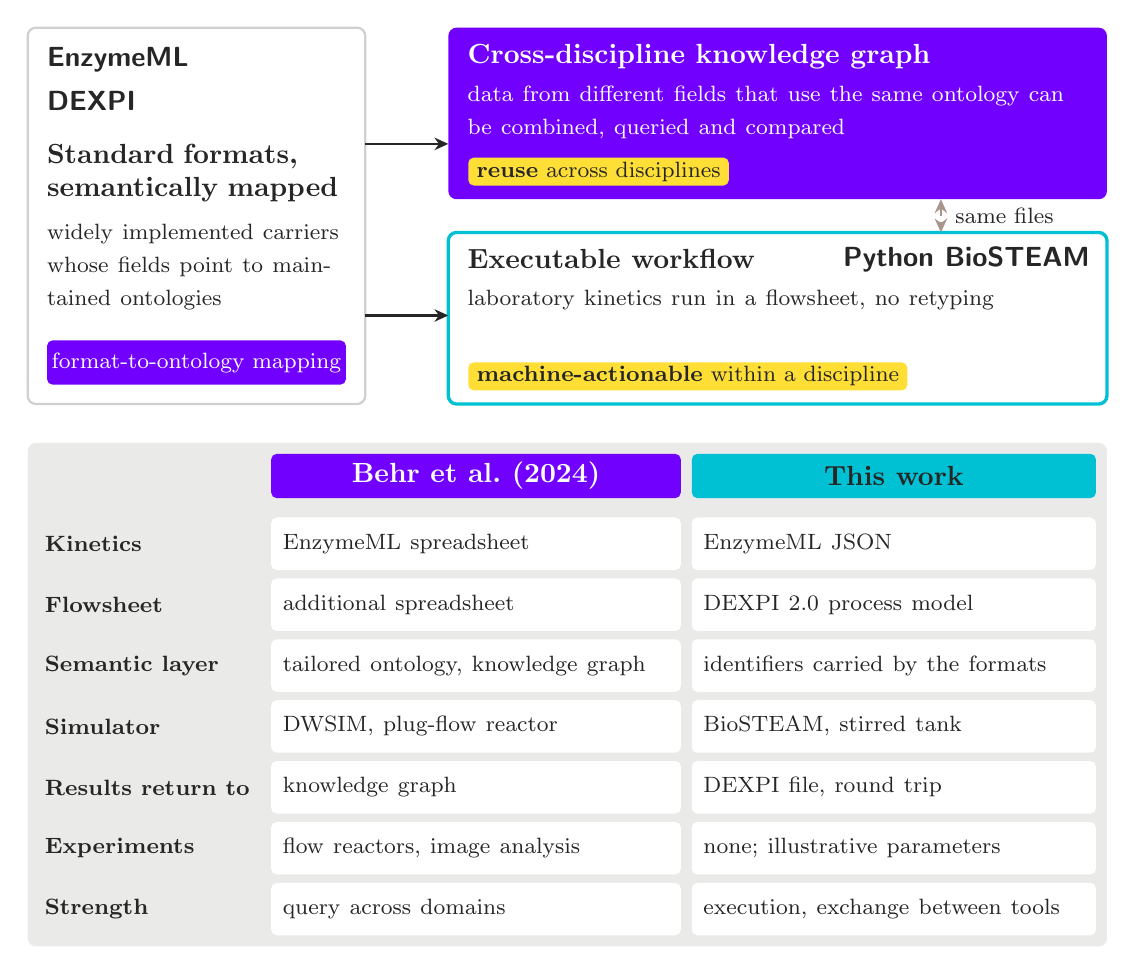
\begin{tikzpicture}
\useasboundingbox (0,0) rectangle (390,332);

% --- source ----------------------------------------------------------------
\draw[card] (0,196) rectangle (122,332);
\node[lbl] at (7,325) {\logo{enzymeml}{11pt}{EnzymeML}};
\node[lbl] at (7,309) {\logo{dexpi}{11pt}{DEXPI}};
\node[lbl, text width=108pt] at (7,290)
  {\hl{Standard formats,\\semantically mapped}};
\node[lbl, text width=108pt] at (7,261)
  {\tx{widely implemented carriers whose fields point to maintained
       ontologies}};
\fill[tuhhpurple, rounded corners=2pt] (7,203) rectangle (115,219);
\node[anchor=center, text=white] at (61,211) {\tx{format-to-ontology mapping}};

% --- route A: knowledge graph ----------------------------------------------
\fill[band, tuhhpurple] (152,270) rectangle (390,332);
\node[lbl, text=white] at (159,326) {\hl{Cross-discipline knowledge graph}};
\node[lbl, text=white, text width=224pt] at (159,311)
  {\tx{data from different fields that use the same ontology can be
       combined, queried and compared}};
\node[tag] at (159,280) {\tx{\textbf{reuse} across disciplines}};

% --- route B: executable workflow ------------------------------------------
\draw[card, draw=tuhhturquoise, line width=1.2pt] (152,196) rectangle (390,258);
\node[lbl] at (159,252) {\hl{Executable workflow}};
\node[anchor=north east, inner sep=0pt] at (384,253)
  {\logo{python}{12pt}{Python}\hspace{4pt}\logo{biosteam}{10pt}{BioSTEAM}};
\node[lbl, text width=224pt] at (159,237)
  {\tx{laboratory kinetics run in a flowsheet, no retyping}};
\node[tag] at (159,206) {\tx{\textbf{machine-actionable} within a discipline}};

\draw[flow] (122,290) -- (152,290);
\draw[flow] (122,228) -- (152,228);
\draw[gap, {Stealth[length=5pt,width=4.5pt]}-{Stealth[length=5pt,width=4.5pt]},
      draw=tuhhwarmgray] (330,270) -- (330,258);
\node[anchor=west, inner sep=2pt] at (333,264) {\tx{same files}};

% --- comparison ------------------------------------------------------------
\fill[band, tuhhcoolgray!45] (0,0) rectangle (390,182);
\fill[tuhhpurple, rounded corners=2pt] (88,162) rectangle (236,178);
\fill[tuhhturquoise, rounded corners=2pt] (240,162) rectangle (386,178);
\node[anchor=center, text=white] at (162,170) {\hl{Behr et al.\ (2024)}};
\node[anchor=center] at (313,170) {\hl{This work}};
\foreach \i/\rowname/\behr/\ours in {
  0/Kinetics/{EnzymeML spreadsheet}/{EnzymeML JSON},
  1/Flowsheet/{additional spreadsheet}/{DEXPI 2.0 process model},
  2/{Semantic layer}/{tailored ontology, knowledge graph}/{identifiers carried by the formats},
  3/Simulator/{DWSIM, plug-flow reactor}/{BioSTEAM, stirred tank},
  4/{Results return to}/{knowledge graph}/{DEXPI file, round trip},
  5/Experiments/{flow reactors, image analysis}/{none; illustrative parameters},
  6/Strength/{query across domains}/{execution, exchange between tools}}{
  \pgfmathsetmacro{\y}{154-\i*22}
  \fill[white, rounded corners=2pt] (88,\y-18) rectangle (236,\y+1);
  \fill[white, rounded corners=2pt] (240,\y-18) rectangle (386,\y+1);
  \node[anchor=west, inner sep=0pt] at (6,\y-8.5) {\tx{\textbf{\rowname}}};
  \node[anchor=west, inner sep=0pt, text width=142pt] at (92,\y-8.5) {\tx{\behr}};
  \node[anchor=west, inner sep=0pt, text width=140pt] at (244,\y-8.5) {\tx{\ours}};
}
\end{tikzpicture}
\end{document}
